In this chapter I will summarize how we can integrate WebRTC with an enterprise collaboration system. I do this by looking at the findings and results from the previous chapters and derive some guidelines. Then in the end I will present a final model of an interworking architecture between the two endpoints.

\section{The enterprise firewall}

\begin{itemize}
\item How do we cross the enterprise firewall?
\end{itemize}
We should configure our SBC or firewall to accept incoming connections from a TURN media relay server as seen in Figure\ref{fig:gateway-final}, and block non-relayed media flows.

\section{The gateway}

\begin{itemize}
\item How can we develop a signaling proxy?
\end{itemize}
On the client side we should implement signaling using a SIP stack with SDP and then transport over a low latency WebSocket connection. Authorization for Kerberos identities should be done using an additional service like the WebAthena proxy. Then in the signaling proxy we should translate messages to whatever is used inside the enterprise system.

\begin{itemize}
\item How can we develop a transport proxy?
\end{itemize}
We should use the open-source RTCWeb Breaker from the webrtc2sip gateway, as it provides everything we need including support for ICE, and encryption/decryption of RTP and RTCP packets. In addition to multiplexing and demultiplexing the streams.

\begin{itemize}
\item How can we develop a transcoder?
\end{itemize}
We should start by implementing the open-source Media Coder from webrtc2sip, but we need to add support for the Theora and Speex codecs as well.

\section{WebRTC mobile client}
When developing a WebRTC client for mobile devices, we should think about signaling and battery consumption. We should create a native client if we want to be able get notified about incoming calls. To be able to get notified, we have to use PUSH notification protocols, because keeping a separate open socket for our application will drain the device's battery. We can download high quality streams, but we may need to send a lower quality upload stream due to lower uplink throughput. Doing multi-party conferencing on low-end devices should be avoided. If the user experiences echo noise issues, he should be adviced to use a headset until the AEC for mobile devices improve.

\section{Interworking architecture}

We see in Figure \ref{fig:gateway-final} that the gateway has evolved throughout this paper. The final model is my suggested approach for integrating WebRTC in an enterprise communication system. In this figure I have included the STUN and TURN server as well. When doing a call from WebRTC to a client inside the enterprise the user will first authenticate his Kerberos identity in the WebAthena proxy, which is not included in this figure. Then he would try to gather ICE candidates from the STUN server. The STUN server will not be able to pass the enterprise firewall, therefore ICE tries to fetch candidates from the TURN server. This works, and the WebRTC client signals the signaling server inside the enterprise with the SDP, by traveling through the signaling proxy. This will negotiate the audio and video codecs, and provide ICE candidates for both clients. The media will then start to be transported, but will be relayed through the TURN server to be able to cross the enterprise firewall. Then the media travels into the gateway where the transport proxy will demultiplex and decrypt the streams, before it continues to transport the media flows to the enterprise media server. If the the media needed transcoding, it would pass through the transcoder first.
\\
\begin{figure}[here]
\centerline{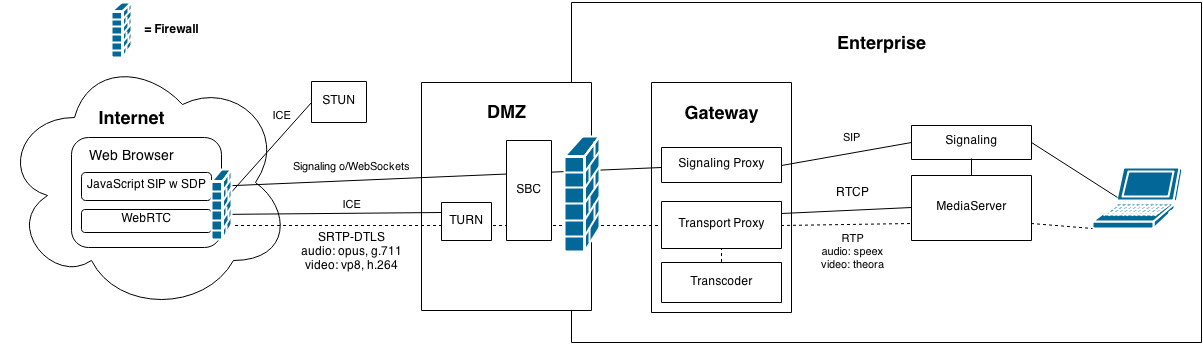
\includegraphics[scale=0.40]{gateway-final.png}}
\caption{WebRTC-Enterpise interworking architecture.}
\label{fig:gateway-final}
\end{figure}


\section{Evaluation}
My proposed solution is pretty similar in architecture to the 3GPPs TR 23.701 mentioned in the background chapter. The main difference is that TR 23.701 does not manage authentication of user identities, and it does not mention anything about media multiplexing. Although STUN is mentioned, there is no explicit mention of TURN support. Since I was not able to create a gateway because of time constraints, I tested some of the components of the webrtc2sip gateway. I found that these worked quite well, and chose to use some of them in my model; the RTCWeb Breaker for the transport proxy, and the Media Coder with support for some additional codecs for the transcoding component.

\section{Summary}
The guidelines provided here are pretty straightforward. However, the authorization part is quite weak, because I have not tested it properly, therefore I chose not to include the WebAthena proxy in the model. I will discuss some missing work for the future in the next chapter. 